\documentclass[10pt]{article}
\usepackage{icmlko}

\icmlmeta{IP 파운데이션 월드모델}{241}{고를 수 없는 이득}{복사본이 준 것은 벌점이 아니라 도메인별 기울기였다 --- 그리고 안쪽은 그것을 거꾸로 고른다}

\begin{document}

\twocolumn[
\icmlheader

\begin{abstract}
노트 240은 ``있는 열을 그대로 복사하면 $+$0.0100 이 난다''를 재고, 그것을
\textbf{그 방향의 능형 벌점이 절반이 된 것}이라고 읽었다. \textbf{그 읽기가
틀렸다.} 복사본에 \emph{하나의} 이름을 붙여 전 도메인이 나눠 쓰게 하면 벌점은
똑같이 반이 되는데 판은 꿈쩍도 안 한다($+$0.0005, $t{=}1.02$). 이득이 나는 것은
\textbf{도메인마다 제 이름을 줄 때}뿐이다($+$0.0102, $t{=}3.07$). 벌점이 아니라
\textbf{도메인별 기울기}다 --- 세 도메인이 \texttt{target\_breadth} 에 공유
계수 위로 자기 기울기를 얹는 것. 손 축 다섯에 다 해 보니 노트 126의 법칙
(``도메인 고유 유연성은 비싸다'')이 \textbf{넷에서 그대로} 지켜진다 ---
\texttt{entry\_friction} 은 $-$0.0309($t{=}-5.40$)다. 그러면 어느 (축, 도메인)
쌍에 기울기를 줄지 \textbf{안쪽에서 고를 수 있나}. 학습 구간을 앞으로 세 조각
내어 41쌍을 다 쟀다. 안쪽 1위는 \texttt{goods\_scale} $\times$ 웹툰(3/3
일치)이고, \textbf{유보 승자는 6 · 7위와 순위권 밖}이며 \texttt{target\_breadth}
$\times$ 웹툰은 부호가 1/3 이라 안정 가드도 못 넘는다. 안쪽이 고른 것을 유보에서
재면 \textbf{$-$0.0070}(3/3 여덟 개를 다 쓰면 $-$0.0077)이고 유보가 고른 것은
$+$0.0100 이다. \textbf{안쪽이 거꾸로 고른다.} 그래서 거부한다 --- 효과가 없어서가
아니라 \textbf{학습 안에서 고를 방법이 없어서}다. 판은 0.4546 그대로 둔다.
\end{abstract}
]

\section{노트 240을 정정한다}

노트 240의 결정적 실험은 이랬다 --- 있는 \texttt{target\_breadth} 열을 그대로
복사해 두 번째 축으로 넣으면 $+$0.0100 이 난다. 새 정보가 0 인데 이득이 나니,
이득은 자료가 아니라 \emph{모형 쪽}에 있다. 거기까지는 맞다.

틀린 것은 다음 한 걸음이다. 나는 그것을 ``그 방향의 능형 벌점이 절반이 된
것''이라고 읽었다. 같은 열이 둘이면 계수를 나눠 가지므로 $\ell_2$ 비용이
반으로 준다 --- 그럴듯하다. 그런데 노트 240의 복사본은 도메인마다 다른 이름을
달고 있었다(\texttt{dup\_tb\_웹툰} · \texttt{dup\_tb\_세계애니} ·
\texttt{dup\_tb\_만화}). 이름을 \emph{하나로} 합쳐 다시 쟀다.

\begin{center}\small
\begin{tabular}{lrr}
\hline
 & F23 판 & 짝 차 \\
\hline
그대로 & 0.4546 & --- \\
복사 · \textbf{이름 공유} · 전 도메인 & 0.4551 & $+$0.0005 ($t{=}1.02$) \\
복사 · \textbf{이름 분리} · 세 도메인 & 0.4648 & $+$0.0102 ($t{=}3.07$) \\
복사 · 이름 분리 · 전 도메인 & 0.4606 & $+$0.0062 ($t{=}1.37$) \\
\hline
\end{tabular}
\end{center}

이름을 공유하면 벌점은 \emph{똑같이} 반이 되는데 아무 일도 안 난다. 그러니
벌점이 아니다. 이득이 나는 것은 도메인이 그 축에 \textbf{자기 기울기}를
가질 때뿐이다 --- 공유 계수는 그대로 두고 그 위에 도메인 전용 기울기를
얹는, 부분 풀링이다.

\section{다섯 중 넷은 손해다}

\begin{figure}[t]
\centering
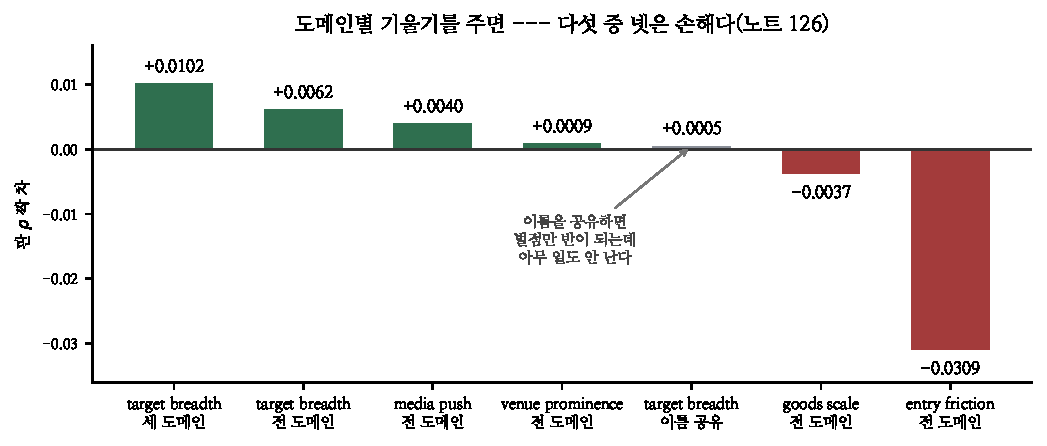
\includegraphics[width=\columnwidth]{figs/slopes.pdf}
\caption{손 축마다 도메인별 기울기를 줬을 때의 짝 차. 이름을 공유하는
회색 막대가 ``벌점이 아니다''를 말한다.}
\end{figure}

손 축 다섯에 각각 전 도메인 기울기를 줘 봤다.

\begin{center}\small
\begin{tabular}{lrr}
\hline
축 & F23 판 & 짝 차 \\
\hline
\texttt{media\_push} & 0.4587 & $+$0.0040 ($t{=}1.75$) \\
\texttt{venue\_prominence} & 0.4553 & $+$0.0009 ($t{=}0.29$) \\
\texttt{goods\_scale} & 0.4514 & $-$0.0037 ($t{=}-1.07$) \\
\texttt{entry\_friction} & 0.4239 & $-$0.0309 ($t{=}-5.40$) \\
\hline
\end{tabular}
\end{center}

노트 126이 잰 ``도메인 고유 유연성은 비싸다''가 그대로 있다. 특히
\texttt{entry\_friction} 은 노트 240에서 모바일 \texttt{price} 를 새 축으로
넣었을 때의 $-$0.0270과 같은 자리다 --- \textbf{그때도 사실은 모바일에게
\texttt{entry\_friction} 전용 기울기를 준 것이었다.} 노트 240은 그것을 ``공유
계수를 빼앗는다''로 적었는데, 더 정확히는 \textbf{빼앗는 게 아니라 갈라지는
것}이고, 갈라지면 대개 나빠진다.

\section{안쪽에서 고를 수 있나}

효과가 진짜라면 남은 질문은 하나다 --- 어느 (축, 도메인) 쌍에 기울기를 줄지
\textbf{유보를 안 보고} 정할 수 있나. 학습 구간을 앞으로 세 조각
(2022 · 2023 · 2024)으로 내어, 관측 80건 이상인 41쌍을 전부 쟀다.

\begin{figure}[t]
\centering
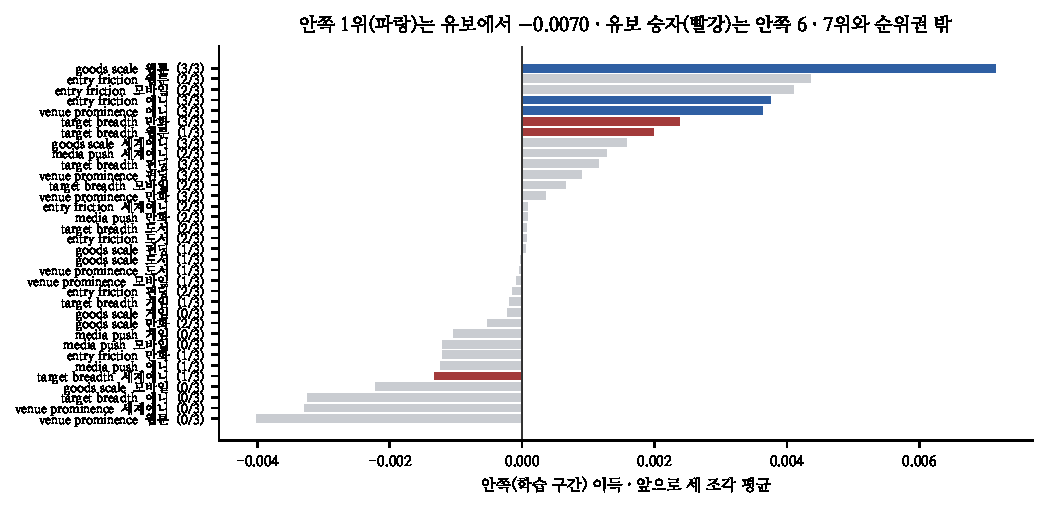
\includegraphics[width=\columnwidth]{figs/innerrank.pdf}
\caption{안쪽 이득 순위. 빨강이 유보 승자 셋, 파랑이 안쪽 1 · 3 · 5위다.
겹치지 않는다.}
\end{figure}

\begin{center}\small
\begin{tabular}{llrr}
\hline
안쪽 순위 & 쌍 & 안쪽 이득 & 부호 \\
\hline
1 & \texttt{goods\_scale} $\times$ 웹툰 & $+$0.0072 & 3/3 \\
2 & \texttt{entry\_friction} $\times$ 웹툰 & $+$0.0044 & 2/3 \\
3 & \texttt{entry\_friction} $\times$ 모바일 & $+$0.0041 & 2/3 \\
6 & \texttt{target\_breadth} $\times$ 만화 & $+$0.0024 & 3/3 \\
7 & \texttt{target\_breadth} $\times$ 웹툰 & $+$0.0020 & \textbf{1/3} \\
--- & \texttt{target\_breadth} $\times$ 세계애니 & \multicolumn{2}{c}{순위권 밖} \\
\hline
\end{tabular}
\end{center}

유보 승자 셋 중 하나는 안쪽 6위, 하나는 7위인데 부호가 1/3 이라 노트 216의
안정 가드를 못 넘고, 하나는 아예 순위권 밖이다. 안쪽 1위는 유보 승자와
아무 관계가 없다.

\section{안쪽이 거꾸로 고른다}

순위만 어긋난 게 아니다. 안쪽이 고른 것을 그대로 채택해서 유보에서 쟀다.

\begin{center}\small
\begin{tabular}{lrr}
\hline
고른 방법 & F23 판 & 짝 차 \\
\hline
그대로 & 0.4546 & --- \\
안쪽 상위 셋 & 0.4476 & $-$0.0070 ($t{=}-1.61$) \\
안쪽 부호 3/3 여덟 개 전부 & 0.4471 & $-$0.0077 ($t{=}-1.66$) \\
\textbf{유보가 고른 셋}(참고) & 0.4648 & $+$0.0100 ($t{=}2.80$) \\
\hline
\end{tabular}
\end{center}

안쪽 선택은 판을 \emph{내린다}. 더 많이 고를수록 더 내린다. 안쪽 신호와 유보
결과가 그냥 약한 게 아니라 \textbf{부호가 반대}다.

\section{거부한다}

$+$0.0102는 재현되는 진짜 효과다. 그래도 안 쓴다. 그것을 쓰려면 어느 세
도메인인지를 \textbf{유보를 보고} 정해야 하고, 그건 유보를 훈련에 쓰는 것이다.
노트 216에서 과제별 혼합 가중($+$0.0050)을, 노트 224에서 웹툰 회차 간격
($+$0.0294)을, 노트 234에서 공유 시리즈 채움을 거부한 것과 같은 이유다 ---
\textbf{판이 올라가는 것과 고를 수 있는 것은 다른 문제다.}

이번 것은 앞의 셋보다 한 칸 더 나쁘다. 앞의 셋은 안쪽이 \emph{못} 골랐고,
이번 것은 안쪽이 \textbf{반대로} 고른다. 그래서 ``나중에 더 좋은 안쪽 규칙을
만들면 되지 않나''도 지금은 근거가 없다 --- 지금 있는 안쪽 신호는 방향
자체가 틀렸다.

\paragraph{남은 것}
\begin{center}\small
\begin{tabular}{ll}
\hline
갈래 & 왜 \\
\hline
안쪽 신호 부호 & 왜 반대인가. 세 조각이 너무 짧은가, 아니면 구조인가 \\
겹말 15쌍 & 시계열 세 축을 하나로 줄이면(노트 240) \\
$\tau$ 칼날 & 잡음 열 하나로 꺼진다. \texttt{STABLE\_MIN} 이 딱 경계 \\
\texttt{media\_push} & 유일하게 도메인별 기울기가 $+$인 손 축($t{=}1.75$) \\
\hline
\end{tabular}
\end{center}

\paragraph{규약에 한 줄 더} 노트 240이 ``새 축은 기존 축과의 도메인 안 순위
상관을 먼저 재라''를 남겼다. 여기에 붙인다 --- \textbf{이득이 났으면 그것이
자료인지 기울기 자유인지 가른다.} 가르는 법은 싸다. \emph{같은 열에 이름을
하나만 주고} 다시 재면 된다. 이득이 사라지면 자료가 아니라 기울기였다.

\end{document}
